% !TEX options=--shell-escape
\documentclass[usenames,dvipsnames,9pt]{beamer}

\usepackage{tikz}
\usetikzlibrary{arrows,shapes,snakes,automata,calc,matrix,backgrounds,petri, positioning}

\makeatletter
\def\input@path{{../support/beamer-template/}}
\makeatother

\usepackage{../support/beamer-template/beamerthememetropolis}

\usepackage[utf8]{inputenc}
\usepackage[czech]{babel}
\selectlanguage{czech}

\usepackage{hyperref}
\usepackage{fontawesome}
\usepackage{minted}
\usepackage{mathtools}
\usepackage{tabularx}
\usepackage{smartdiagram}
\usepackage{soul}
\usepackage{tikz}
\usepackage{amssymb}
\usepackage{qrcode}

% Commands shared between most of the tutorial slides

% Homework deadlines
\newcommand{\hwVIIdeadline}{10. 5. 2020}



% Download icon and text with link relative to the root of the courseware site
\newcommand{\download}[1]{\hfill\faDownload\hspace{5pt}\href{https://cw.fel.cvut.cz/wiki/_media/courses/be4m36mas/#1}{\tt #1}\\[1.3em]}

% Draw eye icon
\newcommand{\see}[1]{\faEye\hspace{5pt}#1}

\newcommand{\sep}{\hspace{10pt}/\hspace{10pt}}

\def\Ipe#1{\def\IPEfile{#1}\input{#1}}

% Draw pacman icon
\newcommand{\pacman}[1]{\tikz[baseline=.1em,scale=.6]{
    \useasboundingbox (.02,0) rectangle (.6,.6);
  \draw [fill=#1] (.3,.3) -- ++(25:.3) arc (+25:+335:.3) -- cycle;

}}

% Draw ghost icon
\newcommand{\ghost}[1]{\tikz[baseline=.1em,scale=.5]{
  \draw [fill=#1] (0,0) -- (0,.5) arc (+180:0:.3) -- (.6,0) --
  (.5,.15) -- (.4,0) -- (.3,.15) -- (.2,0) -- (.1,.15) -- cycle;
    \coordinate (eye) at (360*rand:.03);
    \foreach \x in {.17,.43}{
      \fill[white] (\x,.5) circle[radius=.1];
      \fill[black] (\x,.5) ++(eye) circle[radius=.05];
    }
}}

\newcommand{\desc}[2]{
  #1

  \vspace{-0.6em}
  \hfill\begin{minipage}{0.9\linewidth}
    #2
  \end{minipage}

  \vspace{0.2em}
}

\newcommand{\redc}{\tikz\draw[red,fill=red] (0,0) circle (.5ex);}

\newcommand{\greenc}{\tikz\draw[green,fill=green] (0,0) circle (.5ex);}


% Default url for generating QR code with feedback form.
\newcommand{\defaultfeedbackurl}{https://forms.gle/vwbWazEu14w1Kf487}

% Generate frame with QR code to a feedback form.
\newcommand{\framefeedback}[1][\defaultfeedbackurl]{
  \begin{frame}[standout]
    \begin{minipage}{0.4\linewidth}
      \begin{center}
        \textbf{\LARGE Díky za pozornost!}
      \end{center}

      \vspace{3em}

      \raggedleft\small Budeme rádi za Vaši\\zpětnou vazbu! $\rightarrow$
    \end{minipage}
    \hfill
    \begin{minipage}{0.5\linewidth}
      \vspace{4em}
      \centering\qrcode[height=\linewidth]{#1}\\
      \vspace{0.8em}
      \url{#1}
    \end{minipage}
  \end{frame}
}

% Url for generating QR code with feedback form.
\newcommand{\feedbackurl}{https://bit.ly/3dGdawj}

% \newcommand{\download}[1]{\hfill\faDownload\hspace{5pt}\href{https://cw.fel.cvut.cz/wiki/_media/courses/be4m36mas/#1}{\tt #1}\\[1.3em]}
% \newcommand{\see}[1]{\faEye\hspace{5pt}#1}
% \newcommand{\sep}{\hspace{10pt}/\hspace{10pt}}
% \def\Ipe#1{\def\IPEfile{#1}\input{#1}}
%
% \newcommand{\pacman}[1]{\tikz[baseline=.1em,scale=.6]{
%     \useasboundingbox (.02,0) rectangle (.6,.6);
%   \draw [fill=#1] (.3,.3) -- ++(25:.3) arc (+25:+335:.3) -- cycle;
%
% }}
%
% \newcommand{\ghost}[1]{\tikz[baseline=.1em,scale=.5]{
%   \draw [fill=#1] (0,0) -- (0,.5) arc (+180:0:.3) -- (.6,0) --
%   (.5,.15) -- (.4,0) -- (.3,.15) -- (.2,0) -- (.1,.15) -- cycle;
%     \coordinate (eye) at (360*rand:.03);
%     \foreach \x in {.17,.43}{
%       \fill[white] (\x,.5) circle[radius=.1];
%       \fill[black] (\x,.5) ++(eye) circle[radius=.05];
%     }
% }}
%
%
% \newcommand{\desc}[2]{
%   #1
%
%   \vspace{-0.6em}
%   \hfill\begin{minipage}{0.9\linewidth}
%     #2
%   \end{minipage}
%
%   \vspace{0.2em}
% }
%
% \newcommand{\redc}{\tikz\draw[red,fill=red] (0,0) circle (.5ex);}
% \newcommand{\greenc}{\tikz\draw[green,fill=green] (0,0) circle (.5ex);}

\title{Globální stav distribuovaného systému}
\date{}
\institute{B4B36PDV -- Paralelní a distribuované výpočty}

\metroset{block=fill}

\begin{document}
\maketitle

\begin{frame}
  \frametitle{Osnova}
  \begin{itemize}
   \item Opakování z minulého cvičení\\[1.5em]
    \item Globální stav distribuovaného systému
    \item Chandy-Lamportův algoritmus\\[1.5em]
    \item Konzultace semestrální práce
  \end{itemize}
\end{frame}

\section{Opakování z minulého cvičení}

\begin{frame}[standout]
 \Huge
 \url{http://goo.gl/a6BEMb}
\end{frame}

{\setbeamertemplate{frame footer}{\see{\url{http://goo.gl/a6BEMb}}}
\begin{frame}[fragile]
\frametitle{Klientské požadavky}

\begin{center}
{\bf Jakým způsobem Raft zpracovává klientské požadavky?}
\end{center}

\vspace{2em}

{\em Zvolte, které z následujících možností platí}

\begin{itemize}
\item všechny požadavky splní
\item splní jen požadavky, které leader klientovi potvrdí
\item splní jen požadavky, které si zapíše do logu nadpoloviční většina serverů
\item potvrzené požadavky může ze svého logu mazat jen nový leader
\item nepotvrzené požadavky si může z logu smazat jakýkoli server
\end{itemize}

\end{frame}


\begin{frame}[fragile]
\frametitle{Role leadera}

\begin{center}
{\bf Jakým způsobem Raft používá leadera?}
\end{center}

\vspace{2em}

{\em Zvolte, které z následujících možností platí}

\begin{itemize}
\item leader má vždy nejvyšší index z běžících procesů
\item kandidát na leadera musí mít nejnovější log
\item pouze leader může posílat požadavky o zápis do logů followerům
\item při výpadku leadera Raft přestane fungovat navždy
\item v systému může být vždy nanejvýš jeden leader
\item systém může být několik epoch bez leadera
\end{itemize}

\end{frame}
}

\section{Globální stav v DS}

\begin{frame}
Detekovat vlastnost systému bývá {\bf zásadní}

\hfill $\rightarrow$ Musíme umět reagovat na události!

\vspace{2em}
\begin{itemize}
\item Nevyužívaná paměť
\item Deadlock
\item Ukončení výpočtu
\item $\dots$
\end{itemize}

\vspace{2em}

V \emph{paralelním systému} již víme jak na to

 \pause\vspace{2em}\hrule\vspace{2em}

  \begin{center}
    \LARGE Jak to vyřešit v případě DS?
  \end{center}
\end{frame}

\begin{frame}
  \begin{center}
    \LARGE Musíme detekovat globální stav systému!
  \end{center}

  \vspace{2em}

  Jak to udělat v jednoduchém synchronním systému?

  \pause\hfill $\rightarrow$ Použijeme fyzické hodiny nebo tiky simulace!

A co když je nemáme?

    \pause\hfill $\rightarrow$ Musíme použít lokální stavy!

      \vspace{2em}\hrule\vspace{2em}

      \begin{center}
    \LARGE Globální stav potom bude sjednocením lokálních stavů\\ $\approx$  řez distribuovaným systémem
  \end{center}

\end{frame}

\begin{frame}

Kdy prohlásíme řez (globální stav) za konzistentní?

\vspace{1em}

\begin{center}
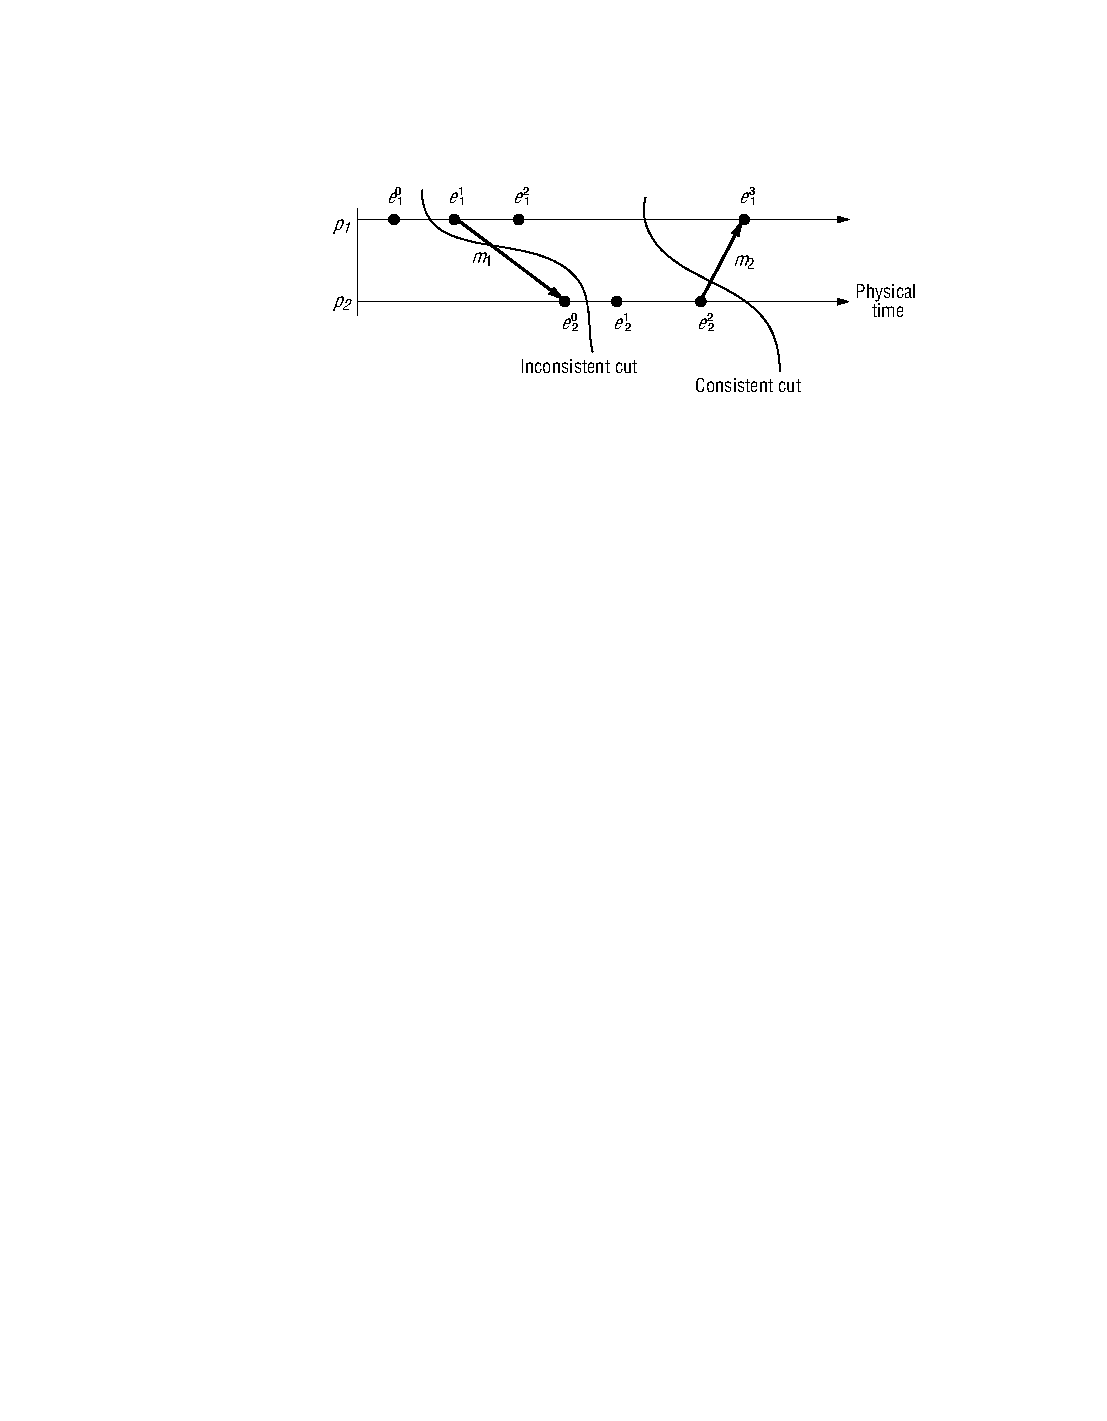
\includegraphics[width=.9\linewidth]{figs/cuts.pdf}
\end{center}

\pause\vspace{1em}

\hfill $\rightarrow$ Musí být splněná kauzalita

\begin{center}
\LARGE Jak vynutit aby globální stav byl vždy konzistentní?
\end{center}

\end{frame}

\begin{frame}
\begin{center}
\large Zaznamenávání lokálních stavů budeme spoustět postupně...
\end{center}
\vspace{2em}
\begin{center}
\LARGE ...prohledáváním do hloubky!
\end{center}
\end{frame}

%\begin{frame}
%
%\frametitle{Požadavky na algoritmy pro globální stav}
%
%Chceme zjistit, zda systém splňuje vlastnost P
%
%U procesů máme opět podobné požadavky jako u vláken
%
%  \begin{itemize}
%    \pause\item {\bf Stability}: když má systém vlastnost P, má ji navždy
%    \pause\item {\bf Safety}: když systém nesplní vlastnost P nyní, nesplní ji ani v budoucnu
%    \pause\item {\bf Liveness}: při jakémkoli běhu systému vždy dojde ke splnění P
%  \end{itemize}
%
%
%\end{frame}

\section{Chandy-Lamportův algoritmus}

\newcommand\snapsize{0.65}
\begin{frame}
\frametitle{Začátek snapshotu}
	\vspace{1.8em}
	\begin{center}
		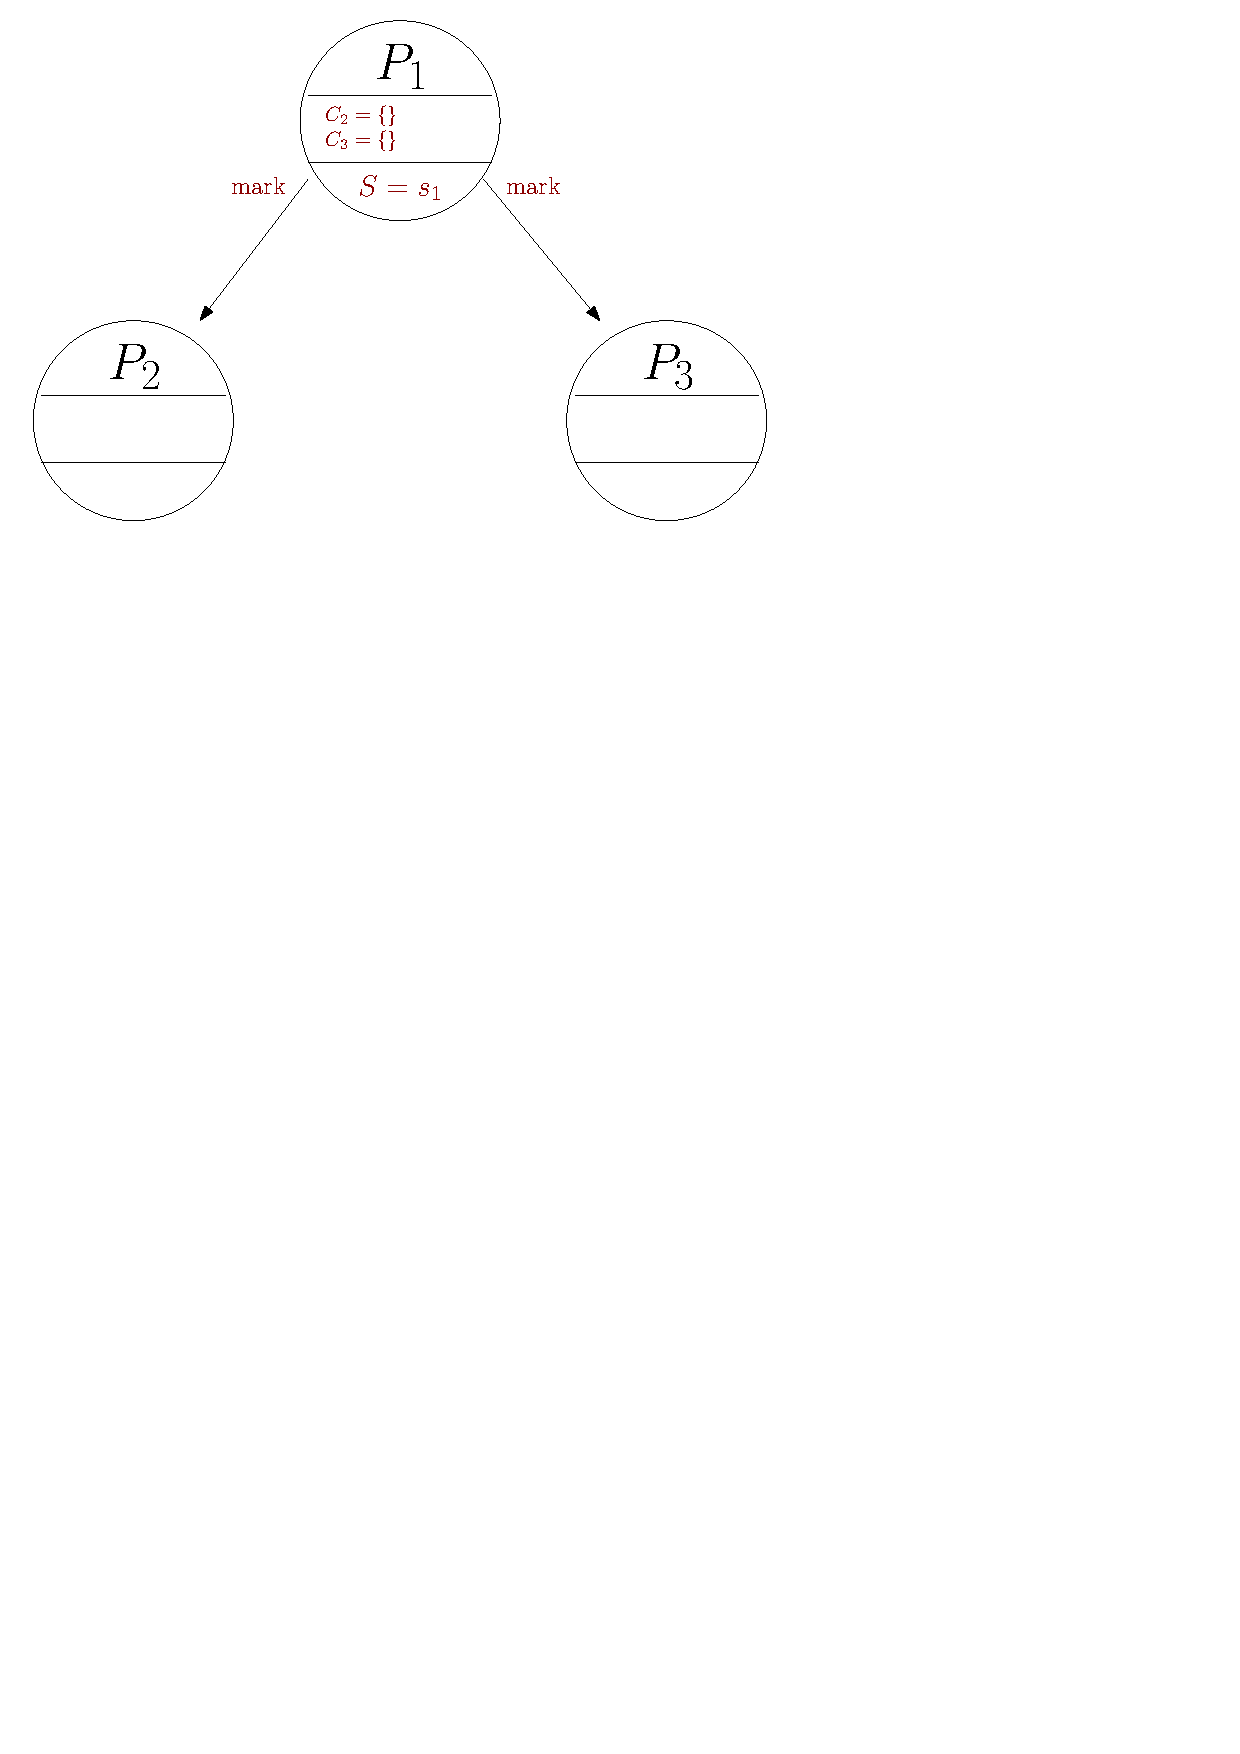
\includegraphics[width=\snapsize\linewidth]{figs/snapshot1.pdf}%
	\end{center}

	{
		\vspace{2em}\hrule\vspace{1em}
		\begin{itemize}
			\item Pokud chce proces $P_i$ začít snapshot, zaznamená svůj stav $S=s_i$, otevře nahrávání zpráv na všech vstupních kanálech a pošle zprávu {\bf mark} všem procesům, se kterými může komunikovat.
		\end{itemize}
	}
	\vfill

\end{frame}

\begin{frame}
\frametitle{Nahrávání}
	\vspace{1.8em}
	\begin{center}
		{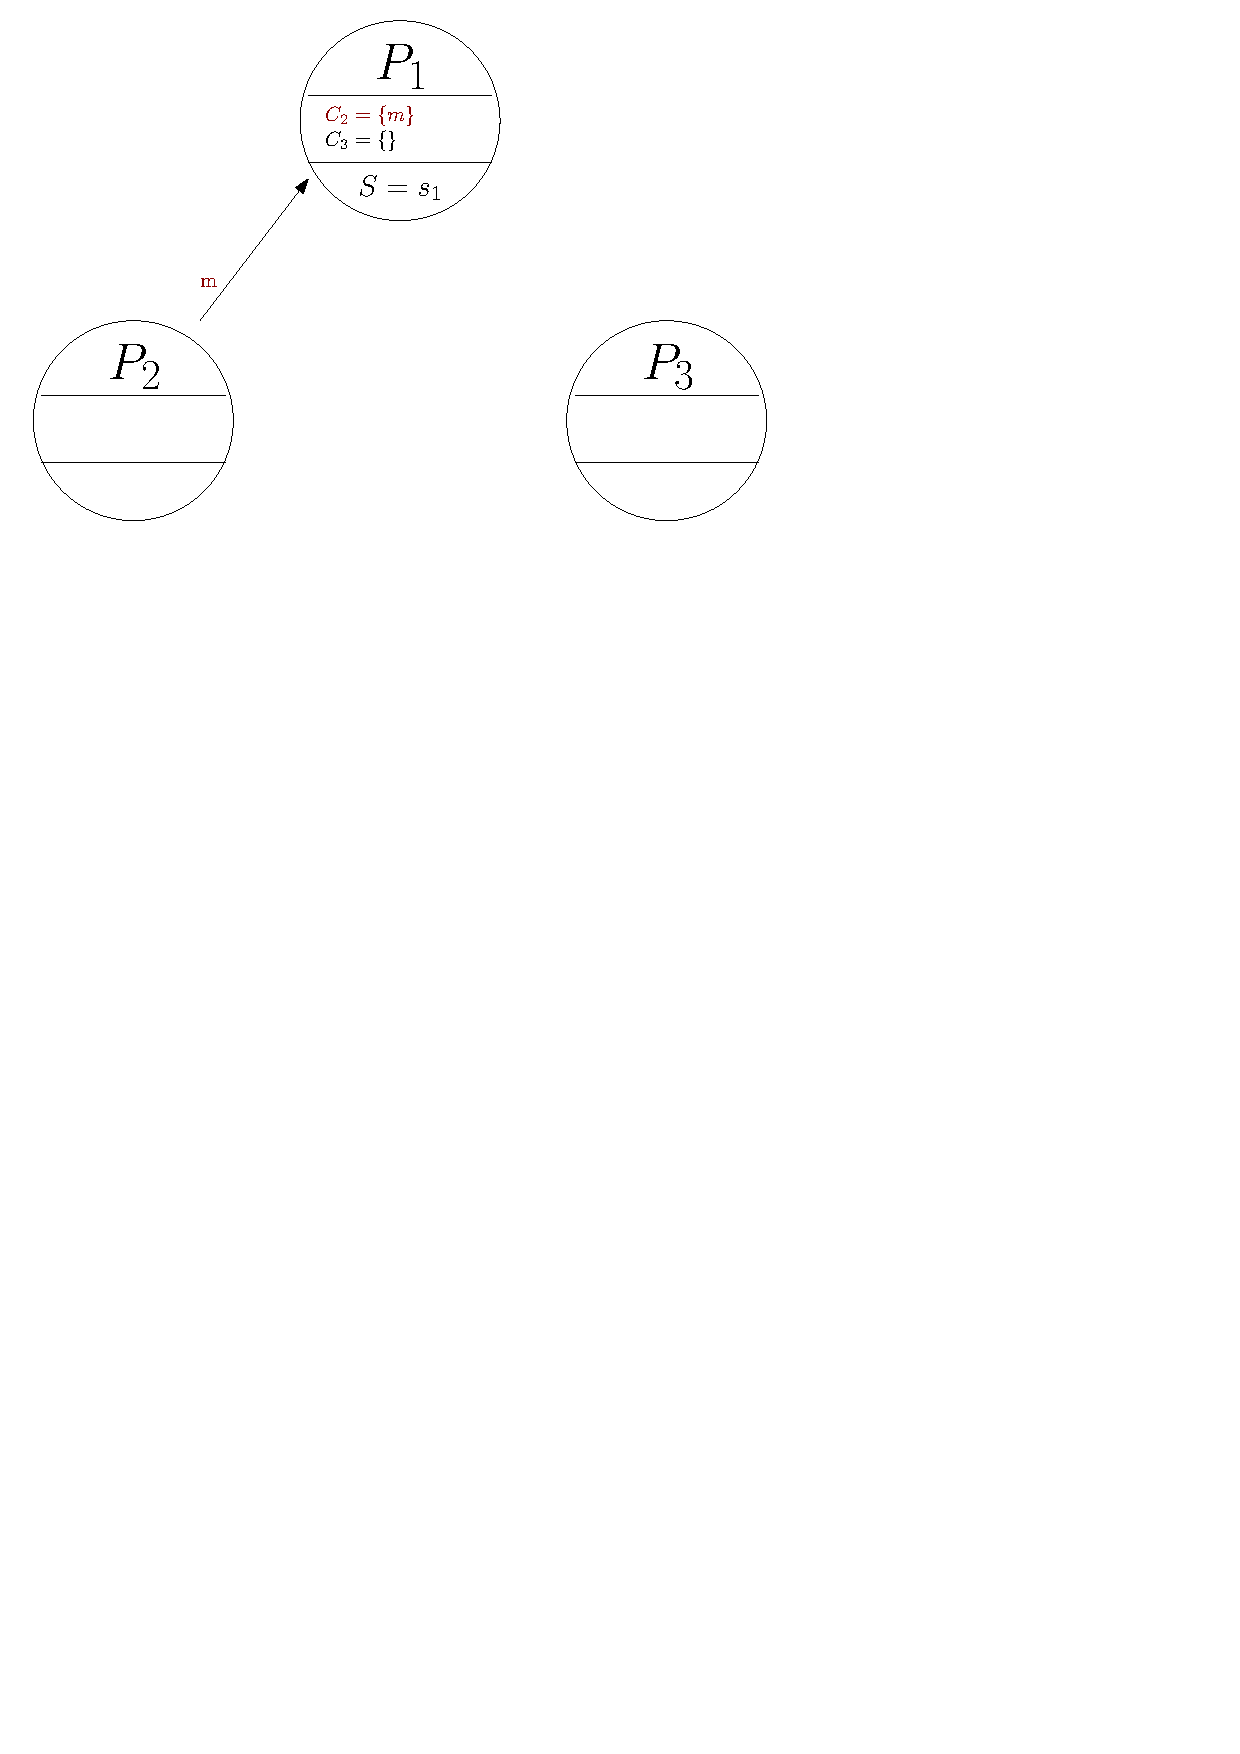
\includegraphics[width=\snapsize\linewidth]{figs/snapshot2.pdf}}%
	\end{center}

	{
		\vspace{2em}\hrule\vspace{1em}
		\begin{itemize}
			\item Pokud proces $P_i$ přijme zprávu po kanálu, který nahrává, tak ji zaznamená.
		\end{itemize}
	}
\vspace{4em}
\end{frame}

\begin{frame}
\frametitle{Příjem markovací zprávy poprvé}
	\vspace{1.8em}
	\begin{center}
		\only<1>{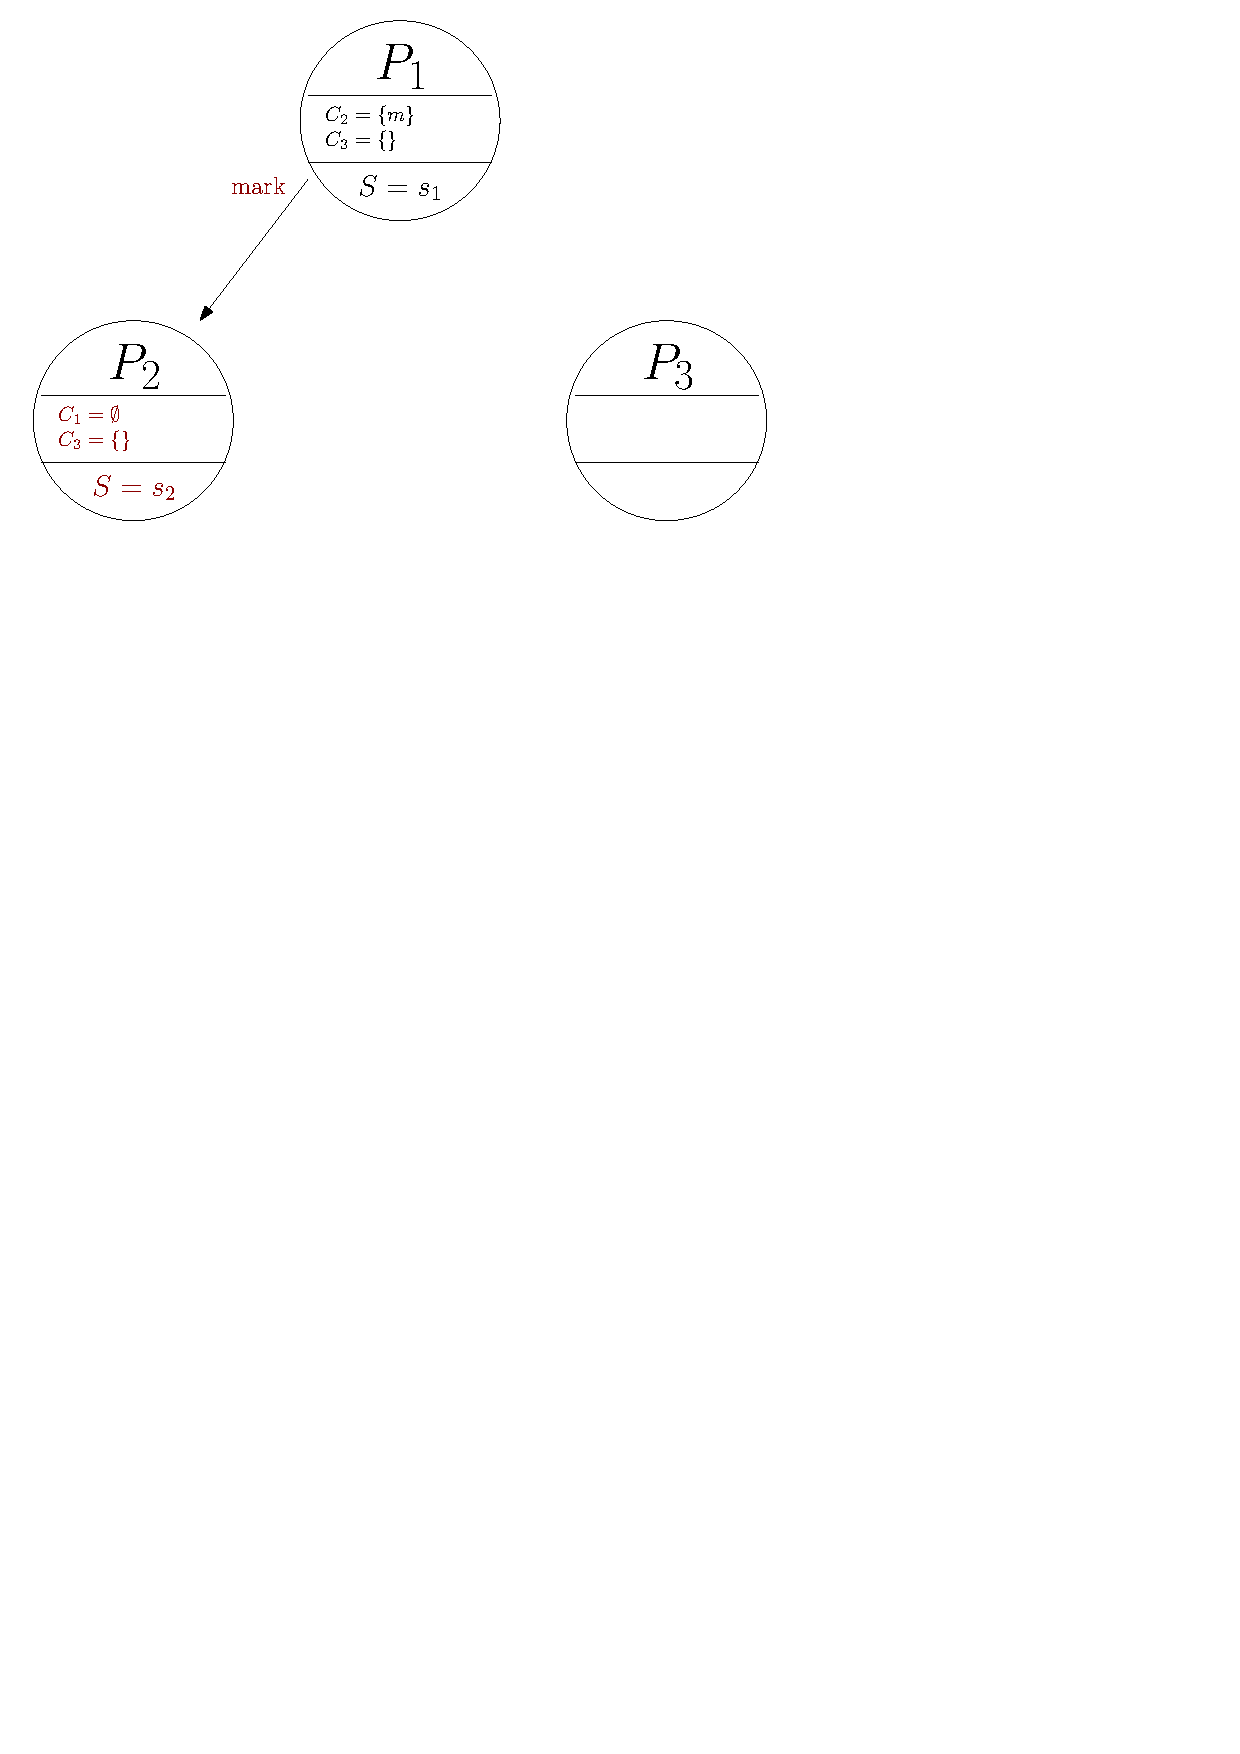
\includegraphics[width=\snapsize\linewidth]{figs/snapshot3.pdf}}%
		\only<2>{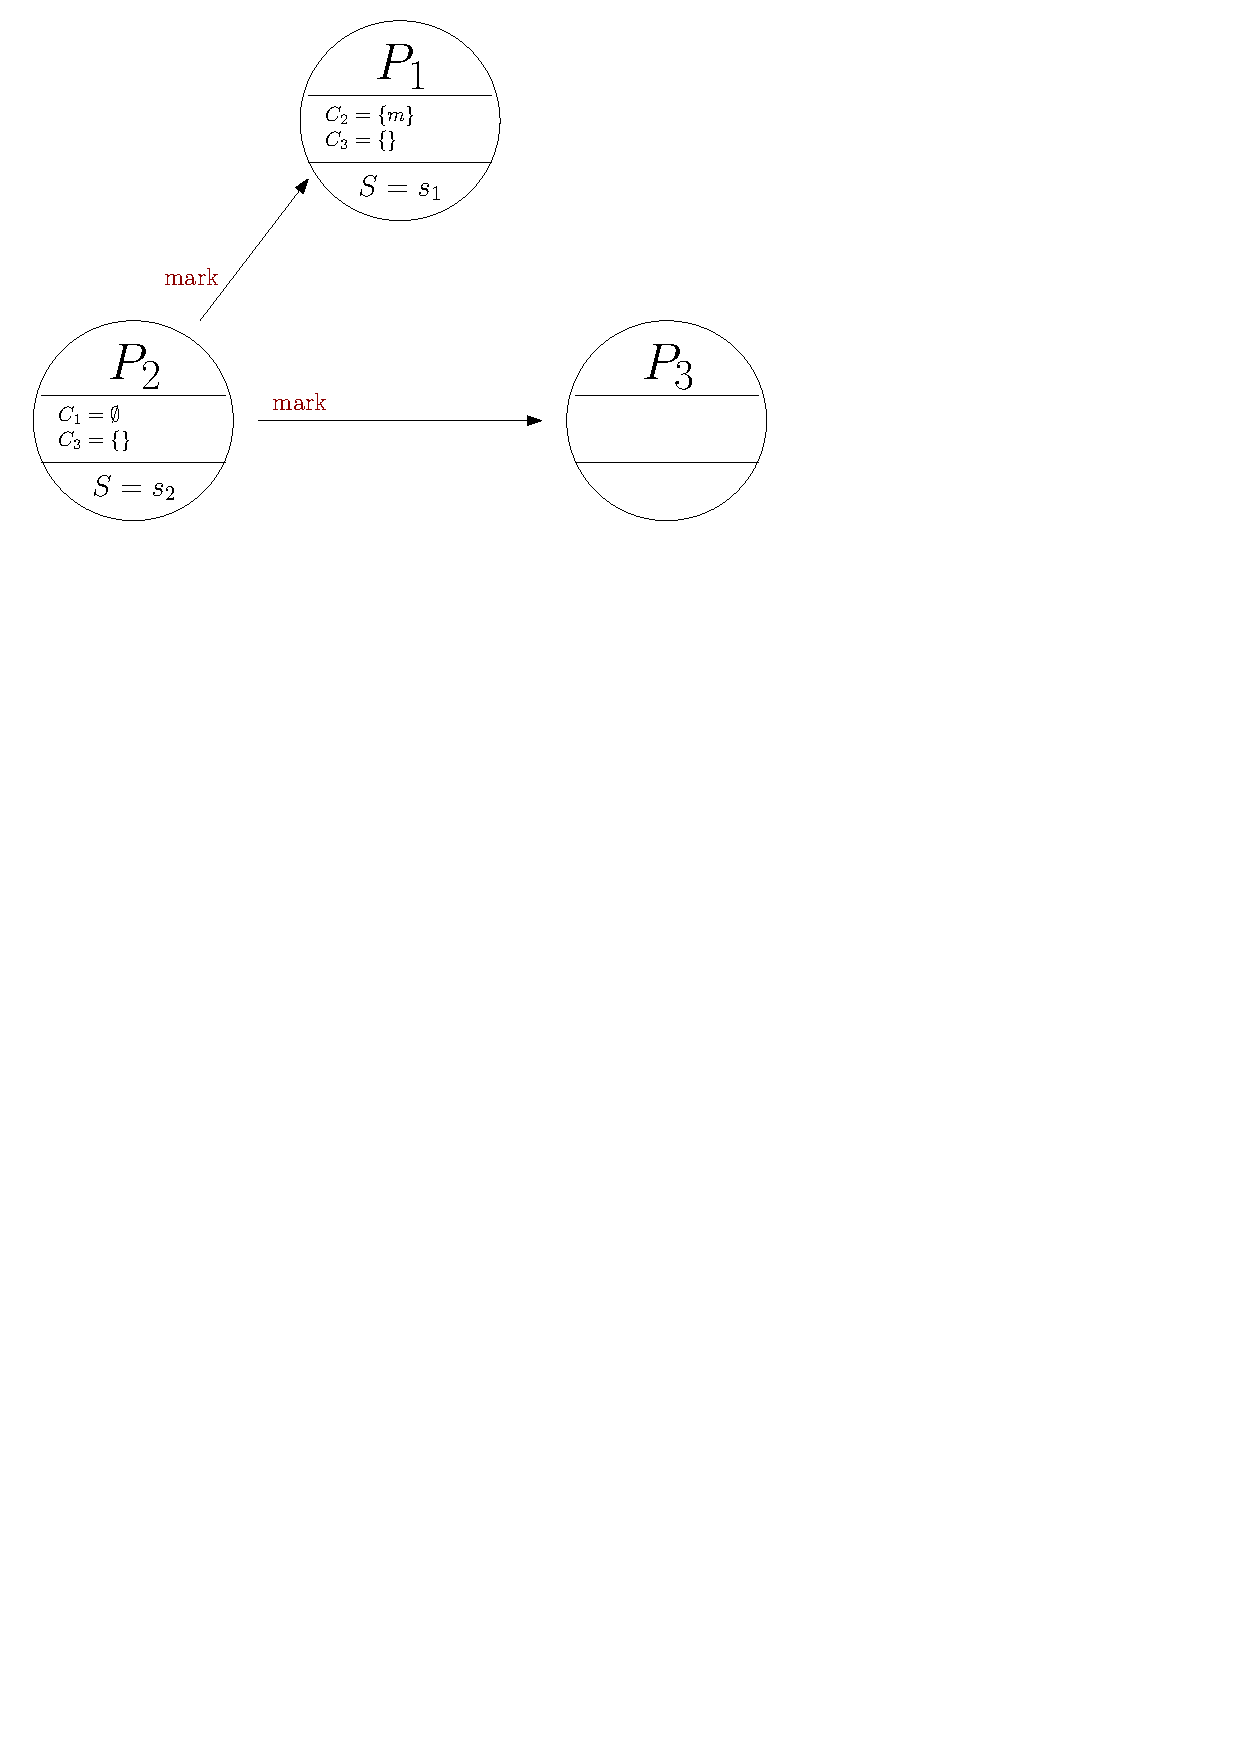
\includegraphics[width=\snapsize\linewidth]{figs/snapshot4.pdf}}%
	\end{center}

{
		\vspace{2em}\hrule\vspace{1em}
		\begin{itemize}
			\item Pokud proces $P_j$ přijme zprávu {\bf mark} a ještě nenahrává, pak zaznamená svůj stav $S=s_j$, otevře nahrávání zpráv na všech vstupních kanálech (krom odesílatele {\bf mark}) a pošle zprávu {\bf mark} všem procesům, se kterými může komunikovat.
		\end{itemize}
	}
\vspace{4em}
\end{frame}

\begin{frame}
\frametitle{Příjem markovací zprávy po nahrávaném kanálu}
	\vspace{1.8em}
	\begin{center}
		{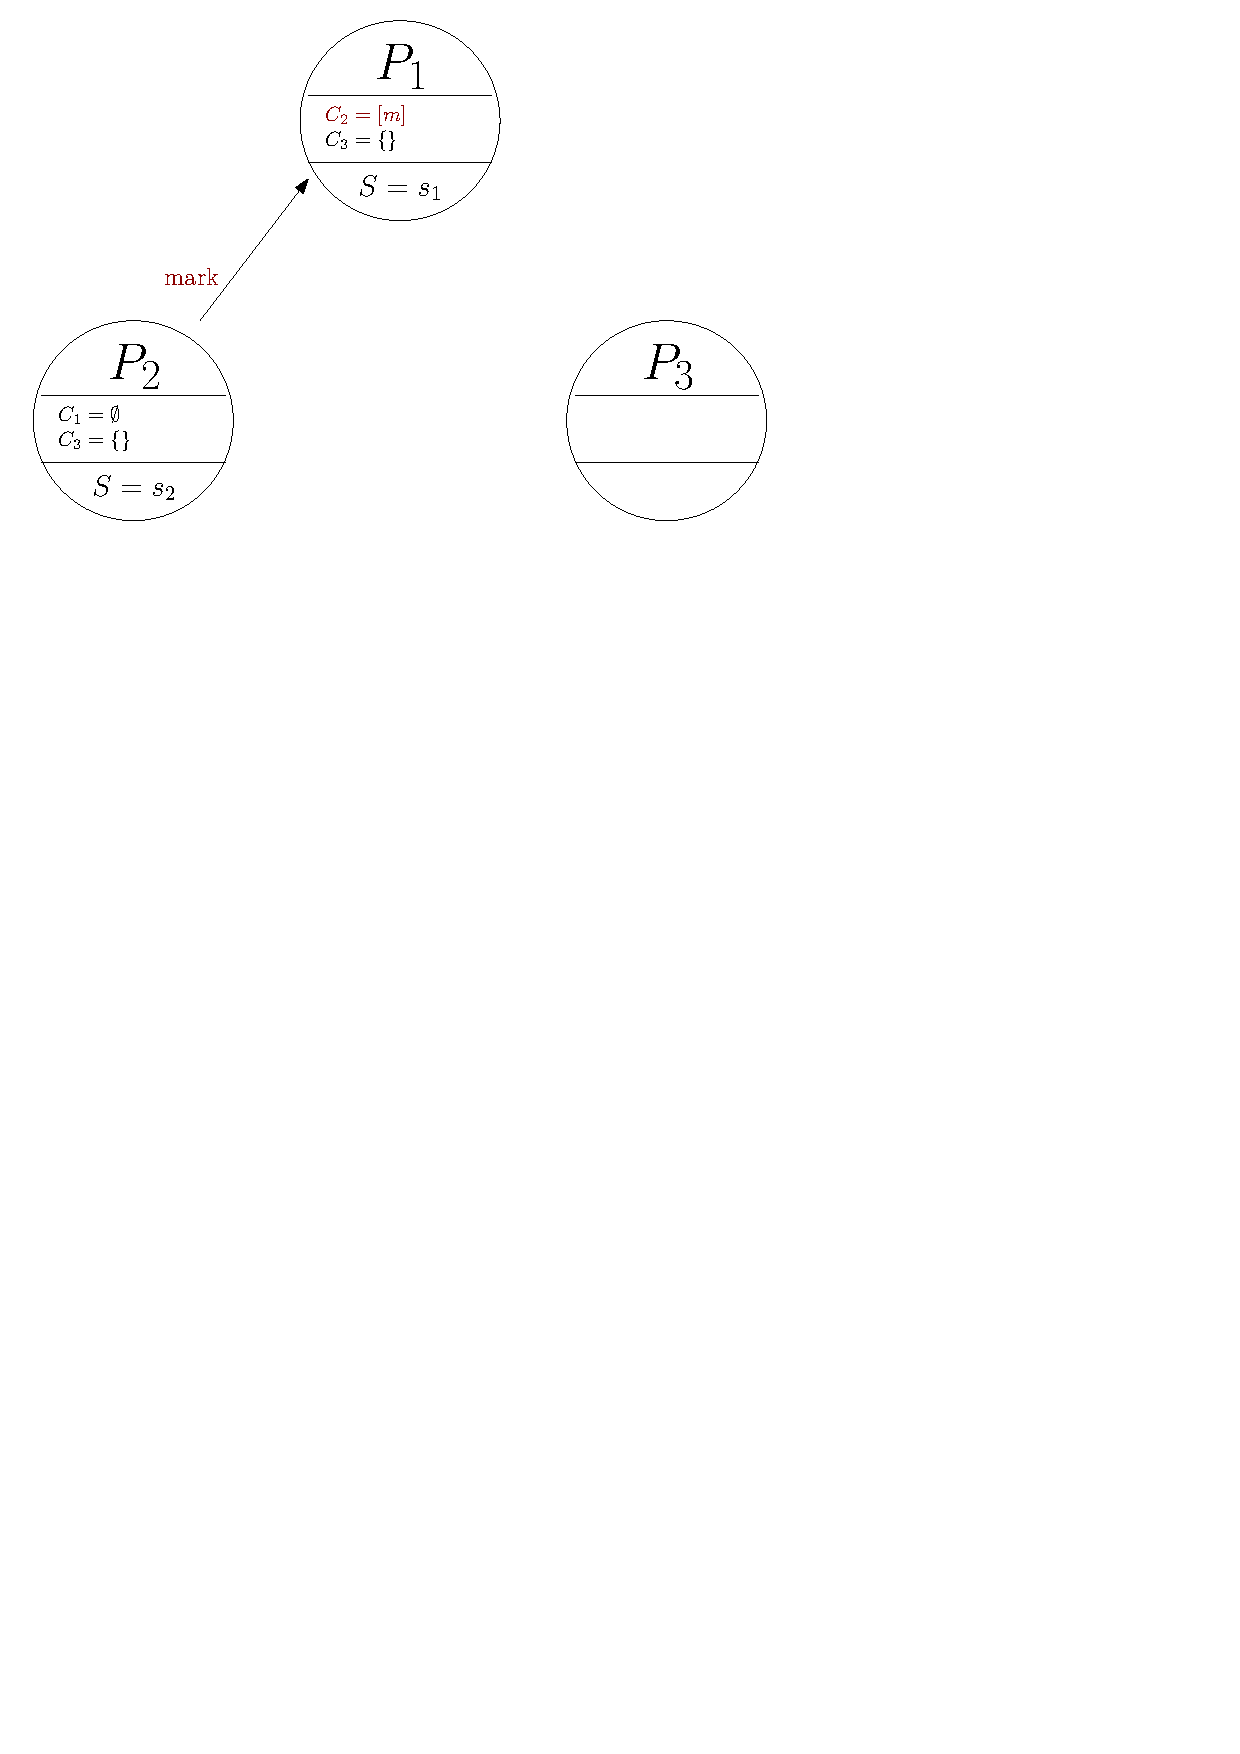
\includegraphics[width=\snapsize\linewidth]{figs/snapshot5.pdf}}%
	\end{center}

	{
		\vspace{2em}\hrule\vspace{1em}
		\begin{itemize}
			\item Pokud proces $P_i$ přijme zprávu {\bf mark} a nahrává, pak nahrávání na tomto kanále ukončí.
		\end{itemize}
	}
\vspace{4em}
\end{frame}

\begin{frame}
\frametitle{Chandy-Lamportův algoritmus}
Když přijde zpráva {\bf mark} od procesu $P_i$
\begin{itemize}
\item Pokud ještě není zaznamenaný lokalní stav: tak ho proces zaznamená a začne nahrávat na všech vstupních kanálech kromě kanálu od $P_i$.
\item jinak: ukončí nahrávání na kanálu od $P_i$.
\end{itemize}

Kdy poslat zprávu {\bf mark}
\begin{itemize}
\item Jakmile proces zaznamená svůj lokální stav, tak pošle zprávu {\bf mark} všem procesům, se kterými může komunikovat.\\ {\small (před tím, než pošle jakoukoli jinou zprávu)}
\end{itemize}
  \vspace{1em}
\begin{block}{Doprogramujte Chandy-Lamportův algoritmus}
    Doimplementujte logiku Chandy-Lamportova algoritmu ve třídě \texttt{snapshot/BankingProcess.java}. Následně spusťte scénář \texttt{bank.Main}.
  \end{block}
\end{frame}

\begin{frame}[standout]
    \begin{center}
      \textbf{\large Díky, že chodíte na cvičení :-)}
    \end{center}
    \vspace{3em}
    \begin{center}
      \textbf{\small Kromě finální PDV ankety vyplňte prosím i}

      \textbf{\LARGE OFICIÁLNÍ ANKETU FEL}
    \end{center}
    \vspace{3em}
     \raggedleft{\small Podle ní jsme hodnoceni fakultou MY}
\end{frame}


% https://goo.gl/forms/DnKuKvur3lsrW4dI3
% AKTUALNI
% \begin{frame}[standout]
%   \begin{minipage}{0.4\linewidth}
%     \begin{center}
%       \textbf{\LARGE Díky za pozornost!}
%     \end{center}

%     \vspace{3em}

%     \raggedleft\small Pokud nám chcete něco sdělit\\ohledně posledního cvičení $\rightarrow$
%   \end{minipage}
%   \hfill
%   \begin{minipage}{0.5\linewidth}
%     \vspace{4em}
%     \centering
\includegraphics[width=\linewidth]{figs/qr_feedback.png}

%     \raggedleft\url{https://goo.gl/forms/DnKuKvur3lsrW4dI3}
%   \end{minipage}
% \end{frame}

% Frame with the feedback QR code
\begin{frame}[standout]
  \begin{minipage}{0.45\linewidth}
    \begin{center}
      \textbf{\LARGE Díky, že chodíte na cvičení :-)}
    \end{center}

    \vspace{3em}

    \raggedleft\huge Vyplňte nám prosím\\FINÁLNÍ ANKETU předmětu PDV! $\rightarrow$
  \end{minipage}
  \hfill
  \begin{minipage}{0.5\linewidth}
    \vspace{4em}
    \centering\qrcode[height=\linewidth]{\feedbackurl}\\
    \vspace{0.8em}
    \url{\feedbackurl}
  \end{minipage}
\end{frame}

\end{document}
